\documentclass{beamer}

\usepackage{graphicx}

\usetheme{default}

\usecolortheme[named=white]{structure}
\setbeamercolor{normal text}{fg=white}
\setbeamercolor{background canvas}{bg=black}

\setbeamertemplate{itemize item}{\color{white}$\bullet$}

\setbeamertemplate{frametitle}[default][center]

\setbeamertemplate{navigation symbols}{}

\begin{document}

\begin{frame}
\begin{centering}
\Huge Research Software Engineering 
\end{centering}

\Large
\pause
\begin{itemize}
\item Types of software
\pause
\item Publication economy
\pause
\item Software development practices
\pause
\item Problem / Solutions
\end{itemize}

\end{frame}

\begin{frame}
\frametitle{Types of research software}

\begin{columns}
\column{0.5\textwidth}
\begin{itemize}
\onslide<2->
\item Low-level libraries
\begin{itemize}
\item BLAS, FFTW, LAPACK
\end{itemize}
\onslide<3->
\item Software frameworks and languages
\begin{itemize}
\item Julia, NumPy, ROOT
\end{itemize}
\onslide<4->
\item Specialized simulation software
\begin{itemize}
\item Lab-dependent
\end{itemize}
\onslide<5->
\item Scripts
\begin{itemize}
\item For a publication
\end{itemize}
\end{itemize}

\column{0.5\textwidth}
\begin{columns}
\column{0.5\textwidth}
\onslide<2->
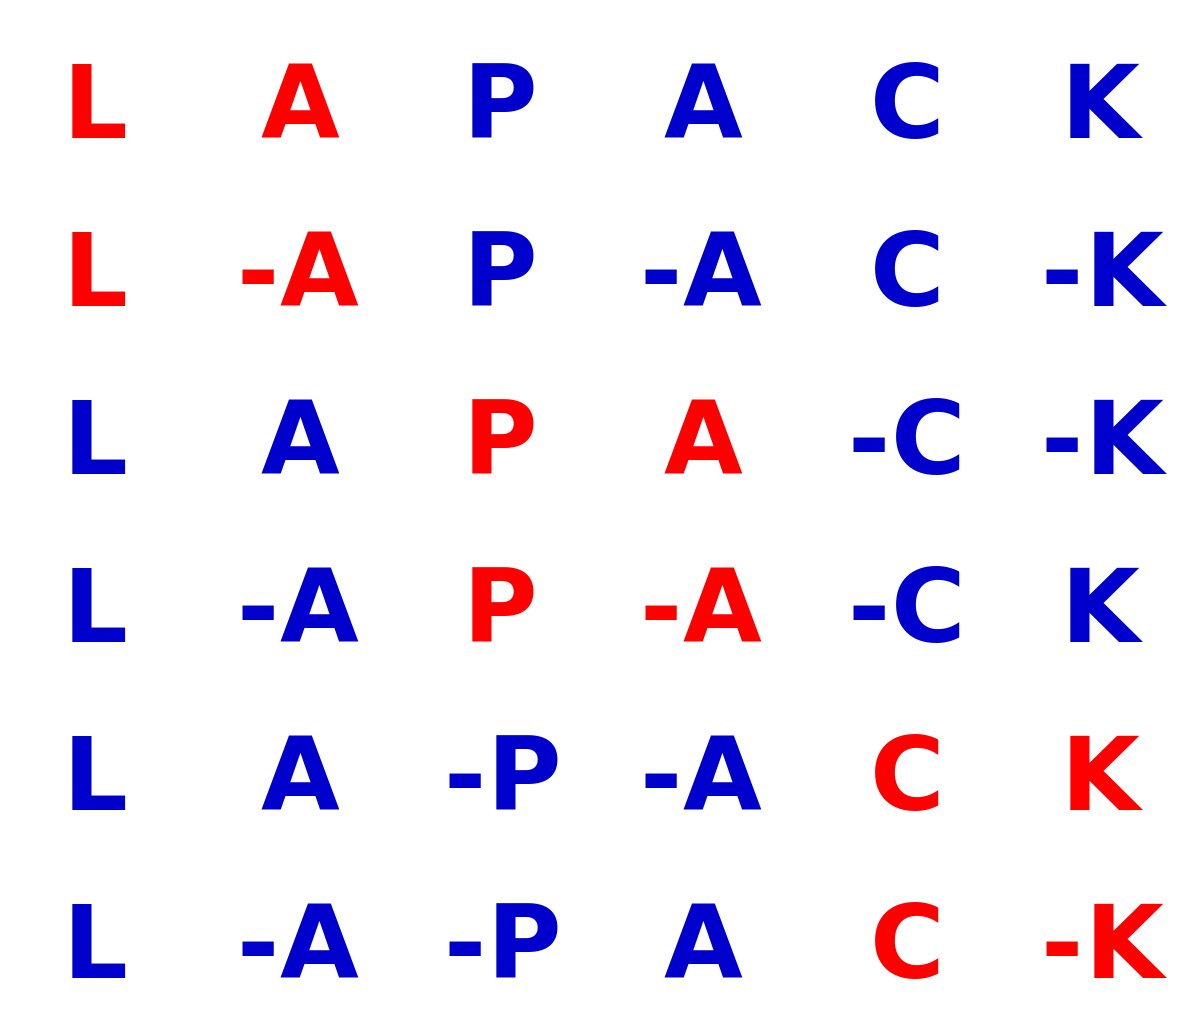
\includegraphics[width=\textwidth]{lapack.png}
\column{0.5\textwidth}
\onslide<3->

\includegraphics[width=\textwidth]{julia.png}
\end{columns}
\begin{columns}
\column{0.5\textwidth}
\onslide<4->

\includegraphics[width=\textwidth]{gpue.png}
\column{0.5\textwidth}
\onslide<5->
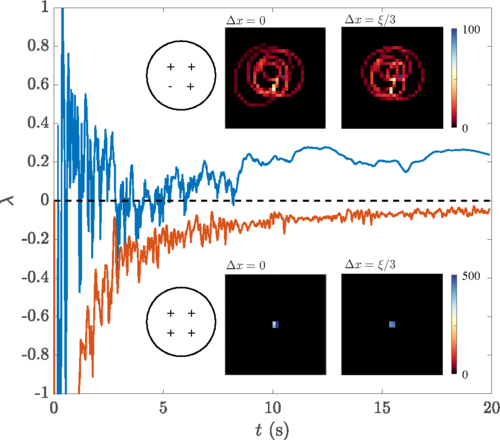
\includegraphics[width=\textwidth]{lyap.png}
\end{columns}
\begin{columns}
\column{0.5\textwidth}
\onslide<4->
\centering [1]
\column{0.5\textwidth}
\onslide<5->
\centering [2]
\end{columns}
\end{columns}
\onslide<6->
\begin{center}
\large Different labs need different software, but most labs need \textit{some form} of software

\onslide<7->
\vspace{0.5cm}
\large Scientific software usually requires some form of domain-specific knowledge
\end{center}
\end{frame}

\begin{frame}
\frametitle{Publication economy}

\begin{columns}
\column{0.5\textwidth}
\onslide<2->
\begin{itemize}
\item Publish or perish
\onslide<3->
\item Code is not reviewed
\onslide<4->
\item Funding
\end{itemize}

\column{0.5\textwidth}
\begin{columns}
\column{0.5\textwidth}
\onslide<2->
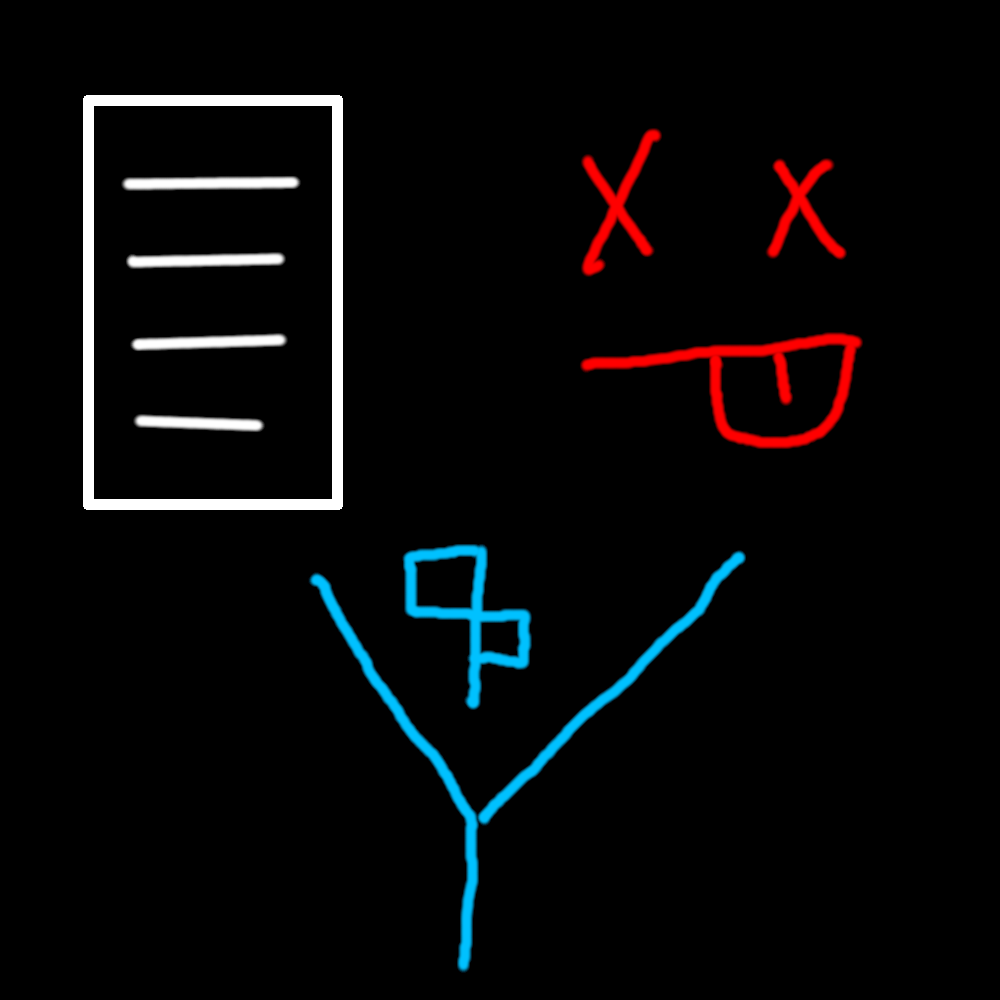
\includegraphics[width=\textwidth]{PP.png}
\column{0.5\textwidth}
\onslide<3->
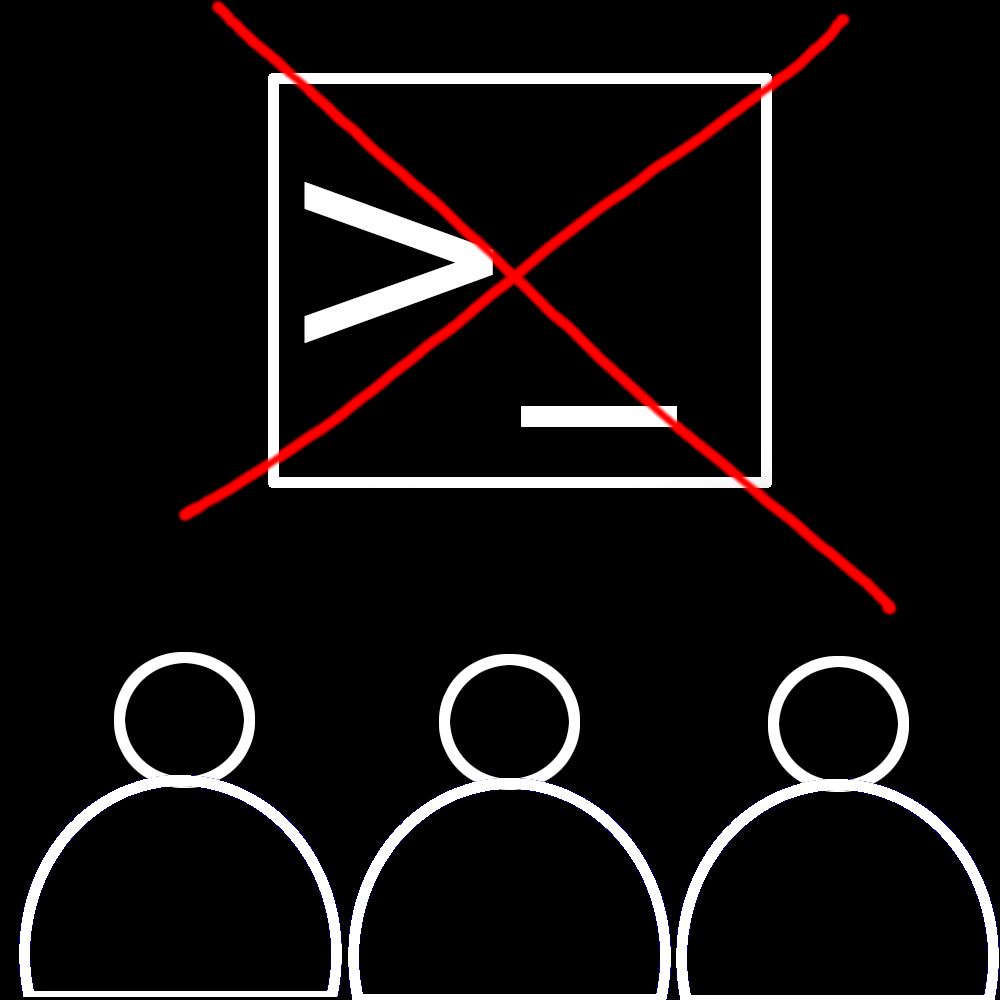
\includegraphics[width=\textwidth]{review.png}
\end{columns}
\onslide<4->
\center 
\includegraphics[width=0.5\textwidth]{money.png}
\end{columns}

\onslide<5->
\begin{center}
\large If results depend on software, this software \textit{must} be robust
\end{center}
\end{frame}

\begin{frame}
\frametitle{Software development practices \\ \small (For those trained \textit{in} academia)}

\onslide<2->
\begin{columns}
\column{0.6\textwidth}
\begin{itemize}
\item The Matlab problem
\begin{itemize}
\item Few functions, structs, loops, include files
\end{itemize}
\onslide<3->
\item No version control
\onslide<4->
\item Little testing, poor documentation
\onslide<5->
\item Little consideration for hardware (High-Performance Computing)
\end{itemize}

\onslide<1->
\column{0.4\textwidth}

\includegraphics[width=\textwidth]{github.png}
\end{columns}

\onslide<6->
\begin{center}
\large Academia does not encourage good software development
\end{center}
\end{frame}

\begin{frame}
\frametitle{Problem Statement}

\pause

\centering \Huge Research Software Engineers are not funded with money or publications
\end{frame}

\begin{frame}
\frametitle{Solutions}

\begin{columns}
\column{0.6\textwidth}

\begin{itemize}
\onslide<2->
\item Journal of Open Source Software
\onslide<3->
\item Fund RSE
\onslide<4->
\item Review code alongside publications
\onslide<5->
\item Embrace open source and contribute back when necessary
\end{itemize}

\onslide<2->
\column{0.4\textwidth}

\includegraphics[width=\textwidth]{joss.jpg}

\begin{columns}
\column{0.5\textwidth}
\onslide<3->

\includegraphics[width=\textwidth]{money2.png}
\column{0.5\textwidth}
\onslide<4->

\includegraphics[width=\textwidth]{review2.png}
\end{columns}
\end{columns}

\onslide<6->
\vspace{1cm}
\centering \Large Headway has been made in all of these areas
\end{frame}

\begin{frame}
\centering \LARGE If scientists are in the business of creating high-quality, replicable scientific results, the software they use \textit{must be} considered part of this process
\end{frame}

\end{document} 
